\chapter{Background}
\label{cha:back}

In this chapter I will cover the context of my project to allow a reader to understand the more complex parts of the report to come.\\
First I will explain the different symptoms that can be felt from hay fever and how they might be caused by different allergens.\\
I will then talk about the main data set used throughout and how I interpreted the data to produce meaninful results.\\

\section{Seasonal Allergies}
A massive 44\% of Britons suffer from at least one allergy, most of those suffering from some kind of seasonal allergy. Allergies are on the rise even with modern allergy medication improving.
\cite{mintelallergy}

\subsection{Asthma}
When talking about hay fever, most assume that it only affects the nose. However, in a study by Eur Respir J. it was found that 20.4\% of allergy sufferers also self-reported suffering from asthma\cite{rhinitis}. By 2025, asthma will represent the most prevalent chronic childhood disease and result in one of the highest health care costs, mainly due to its requirement for ongoing treatment throughout the patients life\cite{childhood}. Despite many decades of research, we do not have a complete solution to the problem. The best we can do it limit exposure, Inhale will help with this by highlighting areas with unsually high occurances of particular symptoms.

Allergy induced asthma causes day-to-day life impacting symptoms. The causes of asthma below clearly indicate allergens and traditional hay fever triggers are also related to asthma causes.\\


\begin{itemize}
  \item Allergens : including pollen, dust mites, animal fur ("dander") or feathers
  \item Airborne Irritants : including cigarette smoke, fumes and pollution
  \item Emotions : including stress or laughter
  \item Weather Conditions : including sudden changes in temperature, cold air, windy days, thunderstorms and hot, humid days
  \item Infections : particularly infections of the upper airways, such as colds and flu
\end{itemize}Adapted from \cite{urlasthmacauses}\\

As you can see, there is a huge variety of factors contributing to allergies. It would be impossible to cover all of these in my one year project. I am going to focus on Airborne Irritants and Allergens.


\section{Britain Breathing}



Here are a couple of mathematical formulae:


A table is just like a figure. Table~\ref{wombat} uses the tabular
environment.  Environments such as tabular can be used in ordinary
text as well.
\begin{table}
\begin{center}
\begin{tabular}{|r|c|c|c|}\hline\hline
place&1991&1992&1993\\\hline
CS Dept& 1&99&199\\
Owens Park& 1876& 22&0\\
Academy&0&0&99999\\\hline\hline
\end{tabular}
\end{center}
\caption{Distribution of Wombats in Greater Manchester}\label{wombat}
\end{table}


\section{Existing Applications}
\label{sec:diagrams}

Figure~\ref{fig:fig-eg} is a figure previously prepared using the
\texttt{xfig} interactive drawing package. With the latest version of
\texttt{xfig} it is quite easy to incorporate \texttt{xfig} diagrams.
The \texttt{xfig} package is menu driven and reasonably self
explanatory.

Use the \emph{Export} menu option to save an encapsulated PostScript
version of your figure, which can then be included in the document
using the \verb=\includegraphics= command. Choose the \emph{Portrait}
orientation option. For example, if the figure is in the file \textsf{
  figure1.fig}, the exporting process will create a file \textsf{
  figure1.eps}, which can then be included, scaled to whatever height
or width you want.


\begin{figure}
\begin{center}
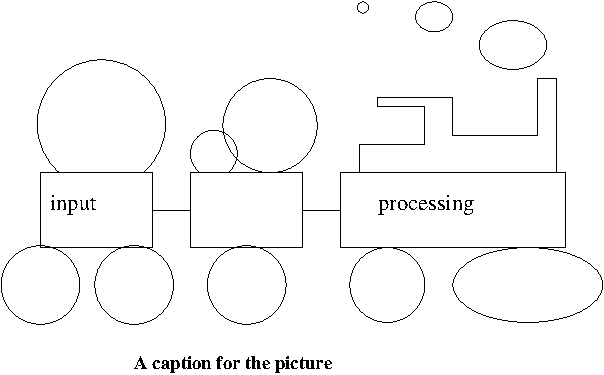
\includegraphics[width=10cm]{figure1} % This scales the picture to
                                      % a width of 10cm
                                      % You can scale to the
                                      % width or height you need
\end{center}
\caption{Final version of the system}
\label{fig:fig-eg}  
\end{figure}

Note that, if you want to use such graphics facilities in some other
document, which does not use either the \texttt{third-rep} or
\texttt{muthesis} document class, you will need to put the command
\verb=\usepackage{graphicx}= after the \verb=\documentclass....=
command in the main file.

\section{Screen Dumps}
\label{sec:screen-dumps}
\begin{figure}
\begin{center}

\includegraphics[width=12cm]{screen}
\end{center}
\caption{A screen dump}
\label{fig:scr-dump}
\end{figure}

Screen dumps can often enhance the appearance and clarity of a report,
although care should be taken not to overuse them. When using screen
dumps it is useful to make use of \LaTeX's capability for using
compressed PostScript files, as in the example shown in
figure~\ref{fig:scr-dump}. 

The image is first captured using, for example, \texttt{xv}, and saved
in a file, e.g.\ \texttt{screen.ps}. Next, extract the bounding box
information from the head of this file. In this case it is
\begin{verbatim}
%%BoundingBox: -100 -16 697 860
\end{verbatim}
and create a file with name given by adding \texttt{.bb} to the
original file name (in this case the name is \texttt{screen.ps.bb}) which
contains just this bounding box. You can now compress the original
file, using \texttt{gzip}. The command
\verb!
\includegraphics[width=12cm]{screen}! will look for either
\textsf{screen.ps} or \textsf{screen.ps.gz}, so you can compress or
uncompress the \textsf{ps} file without changing the latex source.

Alternatively, save as \texttt{.png} if using \texttt{pdflatex}.

The \texttt{draft} option can be used to exclude the actual figure,
but leave an appropriate amount of space.

\textbf{You may not be able to see the screen dump if you are viewing this
file from WWW. This is due to an unfortunate `feature' of the
previewer xdvi.} If you view the files directly from
\texttt{/opt/info/doc/latex/3rd-yr}, things should work properly.

% Local Variables: 
% mode: latex
% TeX-master: "report"
% End: 
